\documentclass[conference]{IEEEtran}
\IEEEoverridecommandlockouts

\usepackage{cite}
\usepackage{amsmath,amssymb,amsfonts}
\usepackage{algorithmic}
\usepackage{graphicx}
\usepackage{textcomp}
\usepackage{xcolor}
\def\BibTeX{{\rm B\kern-.05em{\sc i\kern-.025em b}\kern-.08em
    T\kern-.1667em\lower.7ex\hbox{E}\kern-.125emX}}

%%added
\newcommand{\todo}[1]{{\color{red} TODO: {#1}}}
%% uncomment the following line to make all TODOs invisible in pdf 
%\renewcommand{\todo}[1]{}

\newcommand{\info}[1]{{\color{purple} {#1}}}
%% uncomment the following line to switch \infos back to black 
%% or removing them from the output
%\renewcommand{\info}[1]{{\color{black} {#1}}}
%\renewcommand{\info}[1]{}

\begin{document}

\title{Decode the Work Spouse Code: Investigating the Desired Pair's Role and Pair Programming's Impact on Software Development}


\author{\IEEEauthorblockN{1\textsuperscript{st} Sebastian Sergelius}
\IEEEauthorblockA{\textit{Department of Computer Science} \\
\textit{University of Helsinki}\\
Helsinki, Finland \\
sebastian.sergelius@helsinki.fi}
}

\maketitle

\begin{abstract}
\textit{Context:} Pair programming is often perceived as boosting effectiveness and increasing the correctness of the programming task.
\textit{Goal:} Identify human factors that influence the effectiveness and enjoyment of pair programming, and how they affect the cost and correctness of the task. Understand when, how, and why it is beneficial to do pair programming.
\textit{Method:} A descriptive literature review with aim to categorizing articles whether their title or abstract talks about human factors or quality attributes related to the programming task.
\textit{Results:} A programming partner is expected to have similar traits as your spouse: communicative, open-minded, and complementary skills. Senior pairs do not have significant benefits on effort, duration, or correctness. However, complex software tasks increased the correctness for juniors and intermediate developers. 
\textit{Conclusion:} Pair programming is most efficient for junior programmers doing a complex maintenance task. The study points out that in pair programming it is important to give time to adjust to the situation, remember to communicate constantly, and keep an open mind.
\end{abstract}

\begin{IEEEkeywords}
pair programming, human factors, effectiveness, enjoyment, software quality
\end{IEEEkeywords}

\section{Introduction}

Pair programming has attracted attention in both industry and academia. Pair programming is one of the twelve practices used in Extreme Programming where two programmers work on the same computer aiming to accomplish a software development feature or design \cite{10.5555/1076267}. In a pair programming session, one programmer acts as an observer and the other as the driver. The driver operates the computer, while the observer tries to pinpoint possible defects, think of alternatives, guide the partner with additional resources, or think of the strategic significance of the implementation. Additionally, the roles should be swapped occasionally. Programming is not the only task involved, as pair programming also involves designing and testing the solution. Pair programming has gained interest within the software development industry for its potential to improve software quality, increase productivity, and encourage knowledge sharing, but its practical implementation presents challenges \cite{10.1145/2652524.2652529, Williams2000Strengthening}.

Since pair programming is an interaction between two persons, human factors can cause conflicts or improve productivity. Microsoft researchers surveyed their programmers to discover the various perceived benefits of pair programming in an industry setting \cite{10.1145/1414004.1414026}. According to the respondents, programming in pairs reduces code defects, enhances knowledge sharing, and improves morale and creativity. Problems that the respondents reported were cost efficiency, scheduling, and traits related to individuals, such as personality, skill level, or style differences in programming. 

Even though pair programming has its advantages, its effectiveness is a topic of debate in academia showing mixed results \cite{Hannay2009effectiveness}. Given the growing adoption of agile development methodologies in the software development industry, understanding pair programming benefits and challenges is crucial for knowing when, how, and why to program in pairs. In addition, understanding how it affects software engineering quality attributes, and which quality attributes have been addressed in academia could pinpoint future research directions.

This study reviews empirical studies on pair programming, focusing on perceived benefits and challenges between the pair, and the impact of pair programming on the software quality. The main goal of this study is to identify the human factors affecting the collaboration between the pair, and how pair programming affects the programming task in comparison to programming the task solo.

Section 2 motivates the research topic and discusses the quality attributes under investigation. The third section describes the method used, how the literature was searched, the research questions in more detail, and plans on how to answer them. The result section (Section 4) unveils the characteristics of a desirable partner, and how pair programming affects the cost and correctness of the software. Section 4 discusses the results, implications, and limitations. We end with a conclusion wrapping up the when, how, and why one should consider pair programming.

\section{Background and motivation}

As two persons are assigned to a task instead of one, pair programming has to bring some benefits, otherwise it would be seen as a waste of valuable resources. An answer to the when and why it would be beneficial to apply pair programming, from the perspective of how it affects the overall cost and quality of the software compared to an individual programmer doing the programming task, could strengthen the use cases of pair programming.

One can think of multiple factors that might affect how smoothly the session goes and how they affect the pair programming session \cite{10.1145/1414004.1414026}. The prominent aspect therefore is, what skills and traits are perceived as beneficial from a pair programming partner in comparison to working solo, as the dynamic between the pair play a significant role in the effectiveness of a pair programming session. Additionally, understanding not only the human traits, but whether working environment, equipment or other factors influence a pair programming session. Therefore, identifying these human factors, and to what extent they have been studied would answer when it is beneficial to form a couple. Human factors are not only limited to individual factors, but more broadly to the environment, nature of the task, and organizational factors, such as culture, resources and communication \cite{hseIntroductionHuman}.

Even if an agile team knows when it would be beneficial to work in a pair on a task, a product owner in a team might question why two persons should be allocated for a task instead of one. Therefore, identifying how effective pair programming is crucial helps to argument use cases. The effectiveness of pair programming will be considered by the cost which can be measured by the duration and effort put into the task. Duration is measured from the start of the task to the finish. Related to duration is effort, which is a measurement of pairs combined duration. Accuracy is measured by the correctness of the solution. Studies have measured accuracy with either test cases or a thorough qualitative analysis of the code to find out if there are major defects present. 

\section{Methods}

A descriptive literature review is conducted to provide an overview of existing scientific literature on pair programming based on the published pair programming articles at the Empirical Software Engineering and Measurement (ESEM) conference. This research represents a literature review on the perceived effects of pair programming on the quality of the task, what characteristics are desirable from a pair programming partner, and what is a suitable environment for pair programming, and how these affect the effectiveness and enjoyment of work. 

\subsection{Articles selected}

As the topic is related to empirical evidence on a software practicing technique the reputable ESEM conference is used as the main source for literature. In the ACM Digital Library, the ESEM conference filter is applied, and a search string of "pair programming" is used and should be present in article keywords. A total of four articles were found that were available on the ACM, see first four rows in Table \ref{tab:articles}.

Additionally, each found articles abstract is used as a search string using the free version of Keenious. The highest cited article from the first page of results in Keenious is picked. If Keenious search provided an article already picked on another abstract search, the second highest cited article is picked, and so forth. These articles have inclusion criteria of the abstract mentioning "pair programming". Therefore, we end up with 3 articles from Keenious, see Table \ref{tab:articles}, or \cite{Williams2000Strengthening, Arisholm2007Evaluating, Hannay2009effectiveness}. However, a closer look indicates that \cite{Williams2000Strengthening, Arisholm2007Evaluating} found by Keenious would have been found by snowballing the ESEM articles, and \cite{Hannay2009effectiveness} with backward snowballing. Moreover, the excluded article \cite{ChamorroPremuzic2003Personality} found by Keenious is a reference of \cite{10.1145/1852786.1852816}.

\begin{table*}[]
\caption{Articles selected and categorized that were selected from ACM Digital Library using keyword "pair programming" and ESEM filter, and the four found by Keenious.}
\label{tab:articles}
\begin{tabular}{|p{0.55\linewidth}|c|c|c|c|}
\hline
\textbf{Article [Ref]} & \textbf{Year} & \textbf{\begin{tabular}[c]{@{}c@{}}Citation\\ count\end{tabular}} & \textbf{Human factors} & \textbf{Software quality} \\ \hline
On knowledge transfer skill in pair programming. \cite{10.1145/2652524.2652529}{}                                                   & 2014 & -   & x &   \\ \hline
Pair programming: what's in it for me? \cite{10.1145/1414004.1414026}                                                           & 2008 & -   & x & x \\ \hline
The effects of neuroticism on pair programming: an empirical study in the higher education context \cite{10.1145/1852786.1852816} & 2010 & -   & x &   \\ \hline
An empirical comparison between pair development and software inspection in Thailand \cite{10.1145/1159733.1159749}               & 2006 & -   &   & x \\ \hline
Strengthening the case for pair programming \cite{Williams2000Strengthening}                                                        & 2000 & 794 & x & x \\ \hline
Evaluating Pair Programming with Respect to System Complexity and Programmer Expertise \cite{Arisholm2007Evaluating}             & 2007 & 273 &   & x \\ \hline
Personality predicts academic performance: Evidence from two longitudinal university samples \cite{ChamorroPremuzic2003Personality}       & 2003 & 829 &   &   \\ \hline
The effectiveness of pair programming: A meta-analysis \cite{Hannay2009effectiveness}                                            & 2009 & 235 &   & x \\ \hline
\end{tabular}
\end{table*}

Each article is categorized based on whether either their title or abstract mentions human factors or the quality characteristics of software development. An article can be in multiple categories. Based on the title and abstracts the articles are categorized in the following way: articles \cite{10.1145/2652524.2652529, Williams2000Strengthening, 10.1145/1414004.1414026, 10.1145/1852786.1852816} mentions human factors, and articles \cite{Williams2000Strengthening, 10.1145/1414004.1414026, Arisholm2007Evaluating, 10.1145/1159733.1159749, Hannay2009effectiveness} discusses software quality aspects. The snowballing method for found articles will be applied to additional relevant literature.

\subsection{Research Questions}

Based on the seven found articles and their categorization, this paper seeks to answer the following two research questions.

\begin{itemize}
    \item \textbf{RQ1.} How do human factors influence the effectiveness and enjoyment of pair programming?
    \item \textbf{RQ2.} How does pair programming affect the cost and correctness of the programming task?
\end{itemize}

To answer RQ1 in detail, each of the articles will be evaluated by finding common themes related to human factors, and to evaluate whether the found article discuss these human factors on how they impact the effectiveness or enjoyment of a pair programming session. 

From articles related to RQ2, we try to identify quality attributes that affect the software task when programming in pairs. Whether pair programming leads to higher quality code, whether it improves the time-to-market, and how it compares to individual programming in terms of producing code that meets the requirements, are analyzed from these articles.

\section{Results}

Pair programming has been studied both in industry and in academia \cite{Williams2000Strengthening, 10.1145/1414004.1414026, Hannay2009effectiveness}. Many traits could affect the effectiveness of a pair programming session. Some affecting attributes are personality, skill level, complexity of the task, and the time it takes to adjust to pair programming instead of programming solo (known as "pair jelling"). Furthermore, pair programming can be helpful to reduce the duration of completion of the task, to reduce bugs in the code, and to improve the design of the program \cite{10.1145/2652524.2652529}. In addition, knowledge sharing, focus on the task, improved learning, and building trust within the team are perceived as benefits of pair programming.


\subsection{Human factors affecting a programming partnership}

Pair programming requires more than just software development skills. An essential skill is communication between the pairs. Developers need to be able to provide clear instructions to the pair in case the other pair does not necessarily understand the task goal \cite{10.1145/2652524.2652529}. Furthermore, the receiver of this new knowledge might ask questions that are not related to the task, which requires the responder to focus on the task in progress and possibly deviate from such questions or answer them later after the task is finished \cite{10.1145/2652524.2652529}. Knowledge sharing happens automatically in pair programming sessions, and increases the learning of individuals, however, it requires great communication skills \cite{10.1145/2652524.2652529}. 

With a suitable pair, programmers have reported that they enjoy working more in pairs and they feel more comfortable with their solution \cite{Williams2000Strengthening}. The survey by \cite{Williams2000Strengthening} indicates that 96\% of professionals enjoyed working in pairs more than alone, and up to 90\% of the students agreed. Participants reported that having a partner to bounce of ideas, guide them forward, and finishing the task together gave a feeling of enjoyment. Microsoft programmers answered in their survey that 64.4\% feel that pair programming works for them, and 62.8\% believes it works for their partner \cite{10.1145/1414004.1414026}. Team building is considered a side-effect of pair programming and has been reported to enhance effectiveness and communication \cite{10.5555/377517.377531}. 

Programmers stated that difficulties arise if the other person has a too big or a small ego \cite{Williams2000Strengthening}. With a big ego, the pair does not necessarily have the flexibility to understand that there are multiple ways to accomplish the task. On the other hand, a small ego was perceived as having trouble asserting themselves, and therefore their contribution is low. Similar results were obtained in the Microsoft survey \cite{10.1145/1414004.1414026}. In the survey, the respondents pointed out that problems occur when there are personality clashes, disagreements, programming style differences, or skill differences between the pair \cite{10.1145/1414004.1414026}. Programmers said that unnecessary argumentation, hard to find a consensus in ideas, and that combining different skill levels had a negative impact on the pair programming session. Regarding personality traits, neuroticism in pair programming do not seem to have a significant impact on the effectiveness of a pair programming session \cite{10.1145/1852786.1852816}.

Previous research into pair programming has focused on the duration it takes to accomplish a task \cite{10.1145/2652524.2652529, Williams2000Strengthening, Hannay2009effectiveness}. Williams et al. studied pair programming in academia and showed that working as a pair the task required 60\% more effort, however after the pair had overcome pair jelling, this effort dropped to 15\% \cite{Williams2000Strengthening}. Similar results have been reported by \cite{1541842}, where they noticed that after a few tasks the pairs had a significant drop in the effort to accomplish a task. Additionally, each of the student pairs in \cite{Williams2000Strengthening} handed in the assignment on time, whereas individual students were late or did not hand in the task at all. Moreover, finishing the task boosts the morale and social cohesion of the pair. Working together for a longer period brings up the strengths and weaknesses of the individuals, which increases the effectiveness.


\subsection{The cost and correctness of practicing pair programming}

Previous studies have explored the relationships between pair programming and the time needed to finish the task \cite{10.1145/1414004.1414026, 10.5555/377517.377531, Arisholm2007Evaluating}. The duration is reduced and the correctness of the solution increases. However, the effort (cost) of pair programming a task is higher compared to individuals. Moreover, when taking into account task complexity and expertise, the results vary \cite{Arisholm2007Evaluating}. Nevertheless, with additional manpower, the correctness of the solution is increased or stayed the same.

Earlier mentioned Microsoft survey showed that only a minority (25.4\%) of respondents feel that pair programming takes less time than doing the task alone \cite{10.1145/1414004.1414026}. The biggest perceived benefit of pair programming is code quality and fewer bugs in the code with 65.4\% of respondents indicating so. The most significant problem is cost efficiency. Williams et al. research showed that the used time to complete a programming task dropped by 40--50\% in comparison to individuals \cite{Williams2000Strengthening}. In the same study, they also compared the correctness of the solution by running test cases. All individuals managed to pass under 80\% of the test cases whereas the pairs managed to pass over 80\% of the test cases, even one pair getting up to 94.4\% coverage.


A study compared how expertise and system complexity affected the duration, effort, and accuracy of pair programming a maintenance task compared to individuals \cite{Arisholm2007Evaluating}. Their results show that there was only an 8\% decrease in duration in favor of pairs. However, when taking into account the system complexity, pairs programmed the simple maintenance tasks significantly faster than complex tasks, but with lower correctness. The most significant decrease in duration was seen by pairs of intermediate developers on the simple task with a 39\% decrease in duration, however there was also a 29\% decrease in correctness, see Figure \ref{fig:simple},. In comparison to individuals, the effort required by the intermediate developer pairs for the simple task increased only by 22\%, while juniors with the same task complexity had a significant 109\% increase and seniors 55\%, see Figure \ref{fig:simple}. In the complex task, an increase in correctness was seen by juniors (149\%) and intermediate (92\%) pairs. However, the increased correctness requires significantly more effort, see Figure \ref{fig:complex}. The key takeaway is that simpler tasks had a shorter duration, but were less correct, whereas complex tasks had increased correctness, however, all came with a bigger cost ranging from 22\% for intermediate working on a simple task to 115\% for seniors in a complex task \cite{Arisholm2007Evaluating}.


\begin{figure}
    \centering
    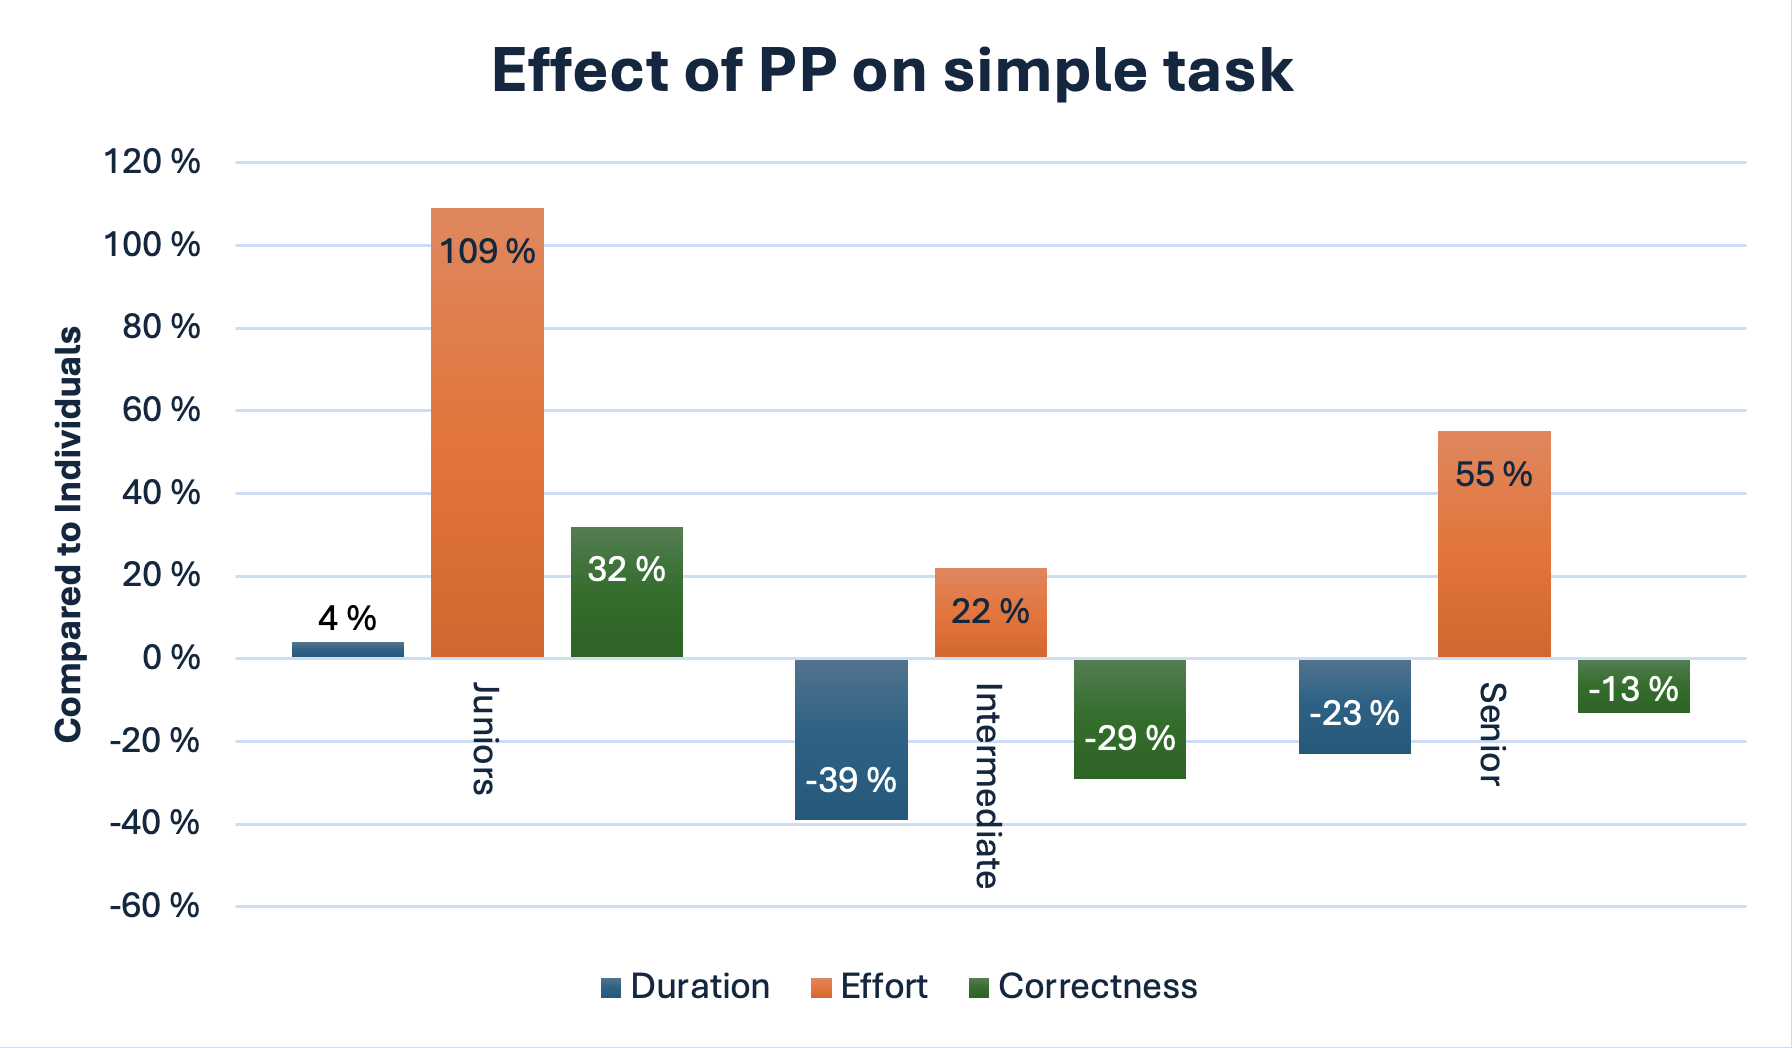
\includegraphics[width=\linewidth]{simple.png}
    \caption{Effect on duration, effort and correctness on a simple task for junior, intermediate and senior developer pairs compared to individuals. Adapted from \cite{Arisholm2007Evaluating}}
    \label{fig:simple}
\end{figure}

\begin{figure}
    \centering
    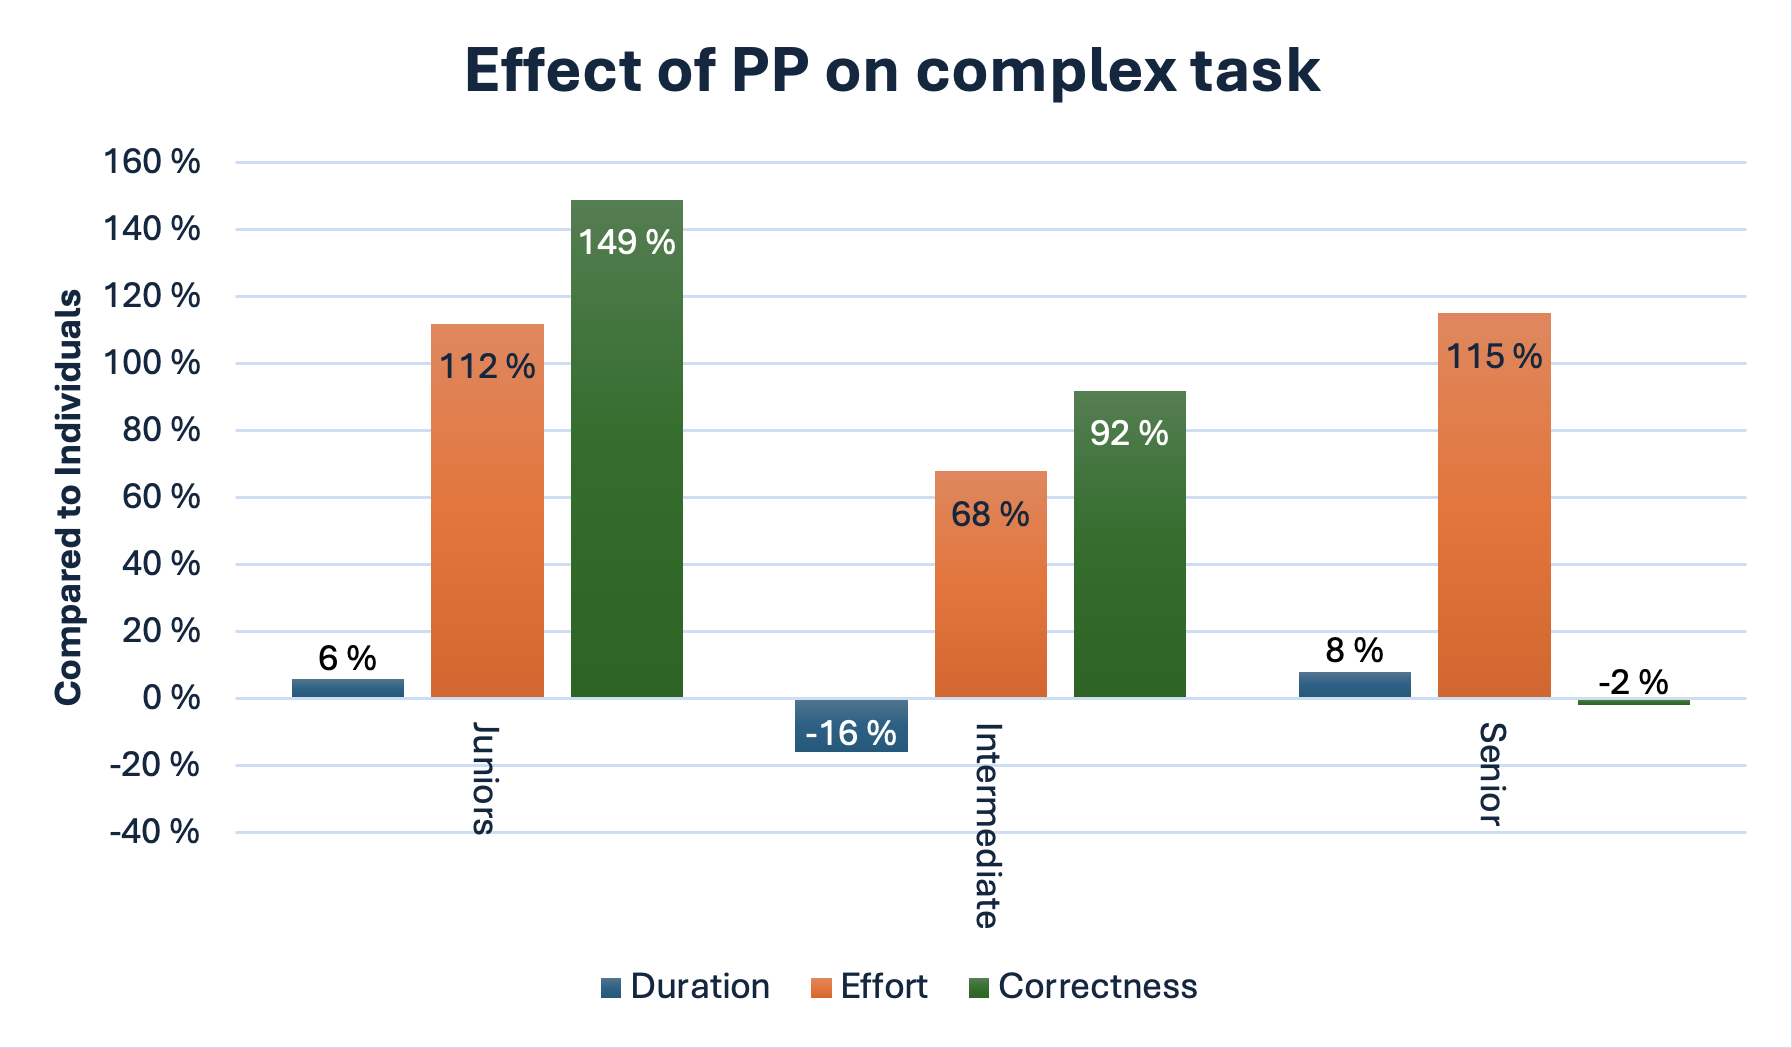
\includegraphics[width=\linewidth]{complex.png}
    \caption{Effect on duration, effort and correctness on a complex task for junior, intermediate and senior developer pairs compared to individuals. Adapted from \cite{Arisholm2007Evaluating}}
    \label{fig:complex}
\end{figure}

The effort invested in pair programming a complex task can reduce the overall cost. IBM reported that they spent 250 million US dollars on fixing 30,000 defects, which converts into 8,000 dollars per defect \cite{10.5555/377517.377531}. Therefore, taking into account quality assurance and other side expenses on defect fixing can reduce the overall cost of the project, as it approximately takes 4--16 hours per found defect for quality assurance engineers. An argument in favor of pair programming by \cite{10.5555/377517.377531}, where they argued that a programmer implements approximately 100 defects per 1000 lines of code (LOC). With a speed of 50 LOC/hour for a 50,000 LOC program, there will be 5000 defects. After code review, approximately 70\% of the defects are found, therefore individuals would have 1500 defects left, whereas pair programmers would have 15\% less (1275) based on their earlier findings in \cite{Williams2000Strengthening}. If a defect takes approximately 8 hours to find and fix, it would take an extra 1800 hours for the quality assurance engineers to fix the program done by individuals. A 50,000 LOC program would take an individual 1000 hours to program, and naively assuming pairs do 50 LOC/hour and doubling the effort for a pair (2000 hours), this would still be in favor of pair programming. 

An experiment was conducted both in academia and industry to understand the effort and correctness of the traditional code and review process compared to doing the whole process during pair programming session \cite{10.1145/1159733.1159749}. The total development cost for pair development, that consists of development and quality assurance, was 4\% higher in an industry setting. However, the software had 39\% less defects compared to the traditional code review team. For undergraduate students and pairs returning a similar quality exercise, showed that the total development cost was 24\% less for the pairs. Reason for the better quality was the early feedback from their partner in both settings. Respondents in a survey said that pair analysis and pair design were seen as more important than pair implementation \cite{Williams2000Strengthening}. Contradicting results are reported in \cite{1541842} that showed there was more defects found by quality assurance persons for pairs in comparison to individuals. However, when taking into account defects found during the coding phase, pairs performed better. In addition, the effort of pair programming in the 400-hour fixed industry experiment showed that pairs had significantly fewer implemented use cases in comparison to individuals \cite{1541842}.

A meta-analysis consisting of 18 studies showed the overall trend on quality, duration and effort on pair programming \cite{Hannay2009effectiveness}. Fourteen of the studies had some form of quality measurement, where only one study reported no improvement in quality. The others reported small to medium improvements. On the duration aspect, eleven studies investigate the duration aspect, and the results show that two showed a negative effect while nine showed a positive effect. The effort was studied in eleven publications, and all except one showed a negative effect on effort. To summarize the trend, most studies show improvements in quality aspects and reduced durations, but with an increased cost (effort). 


\section{Discussion}

This literature review was conducted to try to find an answer to how human factors affect the effectiveness and enjoyment of a pair programming partnership. In addition, the study showed how pair programming affects the cost and correctness of the task. A recap of the results is presented, after which the findings are discussed. 

\subsection{RQ1. How do human factors influence the effectiveness and enjoyment of pair programming}
    
People wish to have a communicative, open-minded, and skillful partner with complementary skills. A big ego is seen as closed-minded, whereas a small ego can be seen as a person being afraid to communicate their thoughts. Personality clashes, disagreements in programming style differences, or skill differences cause problems. The shift from working solo to having a pair is cumbersome, but after a couple of pair sessions, pair programming improved efficiency and enjoyment of work. Focus and discipline for students can be seen by pairs always returning assignments in comparison to individuals. Overall, people enjoy pair programming more than working alone and feel more confident in their work.

In this study, we identified the human factors that influence the pair programming session. However, the question was answered in more of a what form than how human factors affect the effectiveness. Unfortunately, answering the how aspect was not explicitly found in the literature. Most of the studies were surveys based on the perceived human factors a programmer wishes from their partner. Therefore, it can be assumed that these perceived human factors influence the effectiveness and enjoyment of their work. As earlier stated, pairs said that working together boosts confidence that the work done is correct, and that working on simple tasks is better alone. These perceived feelings and understandings from programmers are supported by \cite{Arisholm2007Evaluating}.

When considering that human factors have an impact on the effectiveness, in a small team this could potentially cause conflicts. If two persons feel that they work better as a pair, the others might feel left out or isolated from the team, if the pair always works together. Therefore, there are more aspects on how pair programming builds team cohesion and trust within team. It is important to also rotate the individuals with others in the team to have the benefits of team cohesion. Furthermore, rotating individuals and mixing pairs does increase the knowledge sharing aspect, reducing the risk of having one person knowing it all. Pair programming could be used to get a new team member up to speed faster when knowledge is shared.

Comparing academia and industry, based on \cite{Williams2000Strengthening} and \cite{10.1145/1414004.1414026}, the perceived benefits of pair programming is better in academia. Almost all students felt that pair programming is beneficial, whilst Microsoft engineers were around two thirds. Therefore, pair programming could be more beneficial in academia, especially in a situation of a complex task and students being undergraduates, which could be perceived as junior developers.

    
\subsection{RQ2. How does pair programming affect the cost and correctness of the programming task?}

Different empirical and statistical studies show different results. However, the cost of pair programming depends on the skill level of the pair and the complexity of the task. A junior and intermediate pair benefits from increased correctness, whereas a senior pair does not see similar benefits. On the cost side, the possible reduced duration is mostly balanced out by the used effort of two persons on the task, therefore if shipping the product to market is more important than the cost, pair programming should be applied. Additionally, the increased correctness from programming in pairs can reduce the total price if fewer defects are shipped.

Pair programming research shows that the area of research is enormous, as multiple variables influence the results because we are humans. Therefore, the results of the studies are mixed, as each study has taken into account different aspects. For example, pair jelling was taken into account in Williams et al. study \cite{Williams2000Strengthening}, whereas the larger study conducted by Arisholm et al. in the industry setting did not take into account pair jelling \cite{Arisholm2007Evaluating}.  The variance in effort and correctness of studies show that there are affecting variables that should be taken into account. Therefore, we would need larger studies to get a statistically significant result on how pair programming affects the cost and correctness, with a larger study the other affecting variables would have less of an impact. However, the study setting is hard, as each study might perceive a complex task differently, and also define a junior in their way.

Both \cite{Arisholm2007Evaluating} and \cite{10.1145/1159733.1159749} showed that complex tasks benefit from pair programming in correctness, but it comes with a significantly higher effort, that is the cost is higher. Therefore, if cost and the time-to-market are not an issue, then pair programming is beneficial for complex tasks as it increases the correctness of the solution. Results from a study combining pairs of different skill levels on a complex task would strengthen this insight. In addition, comparing pairs that have worked together and newly created pairs would affect the outcome as \cite{Williams2000Strengthening, 1541842} showed that after a while, the pairs worked significantly faster after they got to know each other and understood how to work in pairs.

Pair programming is beneficial for students, as this adds peer pressure and enhances the motivation to finish the task by the deadline, as it does not affect only the individual's progress in studies as shown by \cite{Williams2000Strengthening}. However, a similar peer pressure effect was not shown in the survey by Microsoft \cite{10.1145/1414004.1414026}. Although it can be argued that if a person enjoys their work more in a pair, it would enhance motivation in the task, so similar to peer pressure in academia to return the assignment in time, we could argue that focus and discipline in an industry setting increase the effectiveness, as it is harder to get distracted if you have a pair that can focus on the task.

Additionally, when conducting pair programming in situations that show improved correctness, with that benefit, and taking into account the amount of possible less defects in the system, the overall cost is hard to measure. However, when considering the reports by IBM \cite{10.5555/377517.377531} on how much they used money to fix defects, and that pair programming had similar effort, but better correctness in \cite{10.1145/1159733.1159749}, these do advocate that pair programming could be an even more cost efficient way of working.

\subsection{Threats to external validity}

Even though studies show that pair programming is perceived as beneficial, and some experiments show good to great results in regards to correctness, duration or effort, these can not be generalized due to the studies being small to medium scale, therefore not statistically significant. Additionally, there is no consensus of what determines a simple and complex task, and what determines if a person is a junior or senior developer.

\subsection{Limitations}

The research method had a limitation when it came to finding relevant literature. Even though the main goal was to identify the perceived characteristics of a desirable pair programming partner, and the affect of pair programming on software quality, searching relevant literature based solely on the ESEM conference increased the odds of missing some relevant literature. Furthermore, the articles presented in ESEM are over 10 years old. In addition, selecting the most cited articles from Keenious might drop out relevant literature as some articles get more citations based on the writer or based on the type of article. Furthermore, citation count grows over time, therefore most cited articles are over 15 years old, and thus there could be more comprehensive studies for the topic under study. Keenious could have provided better results if it was provided with a research plan. Additionally, the literature would have been more broad and not only limited to the ESEM conference.

A second limitation is that almost all of the pair programming experiments involve a small amount of pairs. Therefore, the generalization of whether pair programming is beneficial can not be concluded. The largest statistical study investigated in this paper was \cite{Arisholm2007Evaluating} with almost 100 pairs and 100 individuals. 


\subsection{Future research}

As pair programming is beneficial in a complex task, assuming that complex tasks usually involve some form of larger system knowledge and assuming the longer you work for a company, the more you are aware of the overall system design. A study in an industry setting, where in addition to taking into account the complexity and skill level, taking into account individuals and pair knowledge of the system design or architecture would provide insight into how this knowledge affects the duration, effort and correctness.

In addition, combining different skill levels in the driver and observer seat would also be beneficial. Two seniors are more expensive than one junior and one senior. A study setting like this could have multiple potential perspectives, such as cost, correctness, efficiency, and knowledge sharing aspects.

Human factors in pair programming have been mostly studied from the individual perspective, therefore studies on how other than individual factors, such as how having breaks, swapping the role between observer and driver, or peoples behavior would affect the efficiency of pair programming. Having a more strict process for one pair, and let the other pair work the way they want, could provide insight on the mental load for the observer and driver, and whether having breaks and swapping the role more often has an affect on the effectiveness or quality of the software.

\section{Conclusion}

To conclude, this study was a descriptive literature review of pair programming articles published at the ESEM conference. The goal of this study was to find out what are the desired traits of a pair programming partner, and how pair programming affects the cost and quality of the software. Results show that a desirable programming partner is an open-minded partner with great communication and complementary development skills. By conducting pair programming, knowledge of the software and technical skills are exchanged between the partners, reducing the risk of limiting the information to one person. Pair programming improve the time-to-market when developing complex tasks, and it almost always leads to better results in terms of either the correctness of the solution, or the duration taken to finish. Pair programming requires more effort in man-hours, therefore being more costly. However, the amount of defects found in a task made by pairs is equal or less when compared to individuals, which can lead to significant cost savings when trying to repair these defects in the system later. Considering that money would not be an issue in a software project, working in pairs would brings benefits, such as well-being in work, enhanced knowledge sharing, and increase in the correctness of the solution. No study can pinpoint whether pair programming works for you or your team, the only way to find out is to try it. After each session, reflect on how it went and how you feel. In pair programming, one should remember to be communicative, open-minded, and active. There are no stupid questions.



\bibliographystyle{ieeetr}
\bibliography{refs}

\end{document}
